%% IEEE R10-HTC 2026 -- Special Session 1 "Net Zero Integration"
%% Conference paper, two-column IEEEtran. Compile with pdflatex.
%% Template: https://www.ieee.org/conferences/publishing/templates  (IEEEtran v1.8b, conference mode)
%% Source of record for every number: docs/paper/ieee-r10htc.md  (extended form: docs/paper/draft.md)
\documentclass[conference]{IEEEtran}
\IEEEoverridecommandlockouts
\usepackage[utf8]{inputenc}
\usepackage[T1]{fontenc}
\usepackage{cite}
\usepackage{amsmath,amssymb}
\usepackage{graphicx}
\usepackage{textcomp}
\usepackage{xcolor}
\usepackage{url}

\begin{document}

\title{Open, Reproducible 30\,m Multi-Hazard Flood\\
Screening for Under-Resourced Southeast Asian Cities}

\author{%
\IEEEauthorblockN{1\textsuperscript{st} Daniel Phang}
\IEEEauthorblockA{\textit{[Department --- TBD]}\\
\textit{[Institution --- TBD]}\\
[City, Country --- TBD]\\
0009-0006-3785-4458}
\and
\IEEEauthorblockN{2\textsuperscript{nd} Tze-Houng Lee}
\IEEEauthorblockA{\textit{[Department --- TBD]}\\
\textit{[Institution --- TBD]}\\
[City, Country --- TBD]\\
[email/ORCID --- TBD]}%
}

\maketitle

\begin{abstract}
The Southeast Asian cities most exposed to flooding are precisely those least able
to obtain usable hazard information. The only comparable-resolution (30\,m)
three-hazard model with regional coverage is commercial and closed, and its
free-access tranche explicitly excludes the major ASEAN megacities; bespoke per-city
engineering studies are not publicly reproducible; and the open global products are
an order of magnitude coarser and omit the pluvial (rain-driven) hazard that
dominates urban flooding in the region. We present an open-source, open-data
pipeline that produces design-event coastal, fluvial, and pluvial flood-depth maps
at 30\,m for four cities --- Singapore, Kuala Lumpur, Bangkok, and Jakarta ---
across four ASEAN countries, under four climate combinations (SSP2-4.5 and
SSP5-8.5 $\times$ 2050 and 2100). Every input is freely accessible without
registration, and the pluvial hazard is anchored to the national meteorological
services' published Intensity--Duration--Frequency (IDF) standards, eliminating the
28--62\,\% deficit that global synthetic rainfall carries over tropical-convective
extremes. We make the open model \emph{trustworthy}, not merely reproducible: a
model-blind documented-hotspot location-skill gate yields statistically significant
discriminative skill in all four cities tested, and a bathtub-bias characterisation
(coastal over-prediction of 1.7--25$\times$ at RP100) is closed by a local-inertia
shallow-water solver (Bangkok over-prediction 12.5$\times\rightarrow\approx$1$\times$).
The release is intended as a public good for under-resourced municipal
disaster-management and climate-adaptation agencies.
\end{abstract}

\begin{IEEEkeywords}
humanitarian technology, flood risk, open data, multi-hazard, decision support,
climate adaptation, Southeast Asia.
\end{IEEEkeywords}

\section{Introduction}
Southeast Asia contains six of the ten cities globally most exposed to coastal
flooding by 2100 under high-emission scenarios. Roughly 750 million people live in
the ASEAN region, with about a fifth of regional GDP on flood-exposed
land~\cite{ref_adb}, and the
stressors compound: AR6 P50 sea-level rise under SSP5-8.5 by 2100 ranges from
$+0.62$\,m (Singapore) to $+1.62$\,m (Bangkok); tropical convective rainfall is
intensifying at or above the Clausius--Clapeyron rate~\cite{ref_lenderink}; and
several megacities subside
at 1--25\,cm\,yr\textsuperscript{$-1$} from groundwater extraction and clay
compaction~\cite{ref_abidin,ref_phienwej,ref_chaussard}. The 2011 Thailand megaflood,
the 2020 Jakarta monsoon floods, and the 2021 Kuala Lumpur flash floods are recent
reminders that the exposure is multi-hazard --- coastal, fluvial, and pluvial --- and
concurrent~\cite{ref_hallegatte,ref_tellman}.

Yet the cities carrying this risk cannot readily obtain affordable, usable hazard
maps. Existing flood-screening tools fall into three categories, none of which
simultaneously offers high resolution, multi-hazard scope, open code, open data, and
per-country calibration (Table~\ref{tab:comparator}). The only 30\,m three-hazard
global model is commercial~\cite{ref_fathom}, and its free-access tranche is
restricted to a set of developing countries that \emph{excludes the major ASEAN
megacities}. Bespoke municipal engineering studies exist but are closed and not
reproducible. The open global alternatives are an order of magnitude coarser
($\sim$10\,km) and lack the pluvial layer that drives most urban flood damage in the
region~\cite{ref_hofste,ref_ward,ref_sutanudjaja}. The result is an equity gap: open,
high-resolution, multi-hazard flood information --- a basic input to humanitarian
disaster-risk reduction and adaptation planning --- is unavailable to exactly the
agencies that most need it.

This paper addresses that gap. We present an open-source, open-data,
per-country-calibrated 30\,m multi-hazard flood pipeline and atlas for ASEAN cities,
and --- crucially --- we validate that it locates real floods. The paper covers four
cities (Singapore, Kuala Lumpur, Bangkok, Jakarta) across four countries; two further
cities (Manila, Ho Chi Minh City) are deferred pending a solver extension
(Section~\ref{sec:impact}).

\begin{table*}[t]
\centering
\caption{Comparator landscape for ASEAN-relevant flood-screening tools.}
\label{tab:comparator}
\begin{tabular}{llccccc}
\hline
\textbf{Tool} & \textbf{Resolution} & \textbf{Hazards} & \textbf{Open code} & \textbf{Open data} & \textbf{Per-country IDF}\\
\hline
\textbf{This work} & \textbf{30\,m} & \textbf{C + F + P} & \textbf{Yes} & \textbf{Yes} & \textbf{Yes (4 services)}\\
Fathom 3.0~\cite{ref_fathom} & 30\,m & C + F + P & No & No & Global synthetic\textsuperscript{\dag}\\
Aqueduct Floods 4.0~\cite{ref_hofste,ref_ward} & $\sim$10\,km & C + F & Method only & Yes & None\\
GLOFRIS / PCR-GLOBWB~\cite{ref_sutanudjaja} & $\sim$10\,km & F (+C) & Yes & Yes & None\\
City engineering studies & High & Various & No & No & Per-city\\
\hline
\end{tabular}\\[3pt]
\begin{minipage}{0.92\textwidth}\footnotesize
\textsuperscript{\dag}Fathom's free-access tranche is restricted to selected
developing countries and excludes the major ASEAN megacities covered here --- the
equity gap this work targets. C = coastal, F = fluvial, P = pluvial.
\end{minipage}
\end{table*}

\section{Open Multi-Hazard Pipeline}
\textbf{Open-data inputs.} A per-city configuration drives a single orchestration
script through the pipeline. Every input is free and most require no registration:
the Copernicus GLO-30 DEM (via the Microsoft Planetary Computer), ERA5-Land
precipitation~\cite{ref_era5land} (Open-Meteo), University of Hawaii Sea Level Center
(UHSLC) tide gauges, GloFAS\,v4 discharge reanalysis~\cite{ref_glofas} (Open-Meteo
Flood API), IPCC AR6 sea-level projections~\cite{ref_ar6} (NCAR/Rutgers Zarr), ESA
WorldCover 2021 land cover~\cite{ref_worldcover}, and OpenStreetMap waterways. The
implementation is pure Python on the scientific stack (rasterio, scipy, pyproj,
pysheds, numba); no external binaries or licensed data are required, which is what
makes the pipeline reproducible from scratch by a third party.

\textbf{Per-country IDF anchoring.} The single most important in-region calibration
is the pluvial design rainfall. Global synthetic rainfall statistics under-represent
tropical-convective extremes by 28--62\,\% relative to the national IDF curves, so we
fit a two-anchor Gumbel distribution directly to each country's published design
standard: PUB (Singapore), JPS-MSMA (Malaysia), TMD-RID (Thailand), and BMKG
(Indonesia). The storm duration is matched to the dominant local flood mechanism ---
Singapore uses a 1-hour secondary-drain IDF (its documented flash floods are
sub-hourly convective bursts), the others a 6-hour IDF --- and the post-drain excess
rainfall is the depth the drainage network cannot convey.

\textbf{Three hazards.} \emph{Coastal:} a GEV fit to UHSLC annual-maximum storm-surge
residuals (T\_TIDE-detided~\cite{ref_ttide}), consistent with global storm-surge
reanalyses~\cite{ref_muis2016,ref_muis2020}, plus the AR6 SLR delta, brought onto the
EGM2008 DEM datum via a CMEMS mean-dynamic-topography offset, and routed by a
local-inertia shallow-water solver~\cite{ref_bates} on a staggered grid; a
connectivity-based bathtub solver is retained as a fallback where the sea is enclosed
within the DEM domain. \emph{Fluvial:} GloFAS-derived design stage with bankfull
subtraction for rivers carrying permanent baseflow, mapped via Height Above Nearest
Drainage (HAND)~\cite{ref_nobre,ref_topo} referenced to the \textbf{main-stem trunk the
modelled discharge represents} --- flow-accumulation channels at the GloFAS sub-basin
(catchment) scale rather than a channel-initiation threshold or raw OpenStreetMap
network, which over-broaden the floodplain. \emph{Pluvial:} the IDF excess is routed
by a catchment-routed fill-and-spill cascade~\cite{ref_barnes} (depressions resolved
by a Planchon--Darboux fill~\cite{ref_planchon}) with a per-cell runoff
coefficient from WorldCover land cover, producing a return-period-dependent ponding
extent rather than a uniform cap. The three depth rasters are composited by per-pixel
maximum.

\textbf{Scenarios.} All hazards are produced for SSP2-4.5 and SSP5-8.5 at 2050 and
2100, on a subsidence-corrected DEM (a zone-based correction for the documented
post-2013 subsidence in Jakarta and Bangkok). Per-step methodological detail is
documented and reproducible in the open repository.

\begin{figure}[t]
\centering
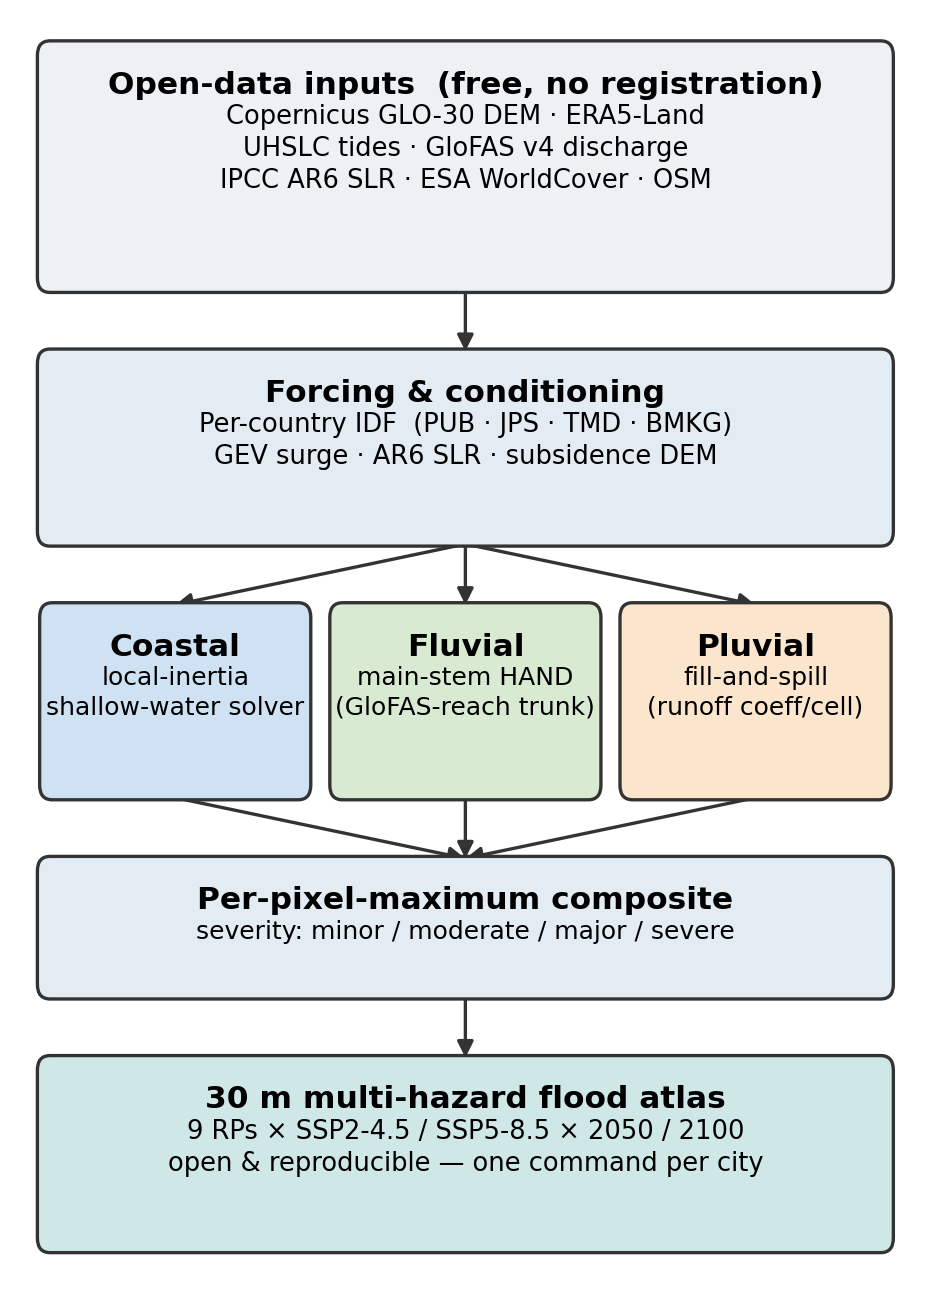
\includegraphics[width=\linewidth]{figures/ieee_fig1_pipeline.png}
\caption{Pipeline data-flow schematic: free open-data inputs $\rightarrow$ per-hazard
solvers (inertial coastal, main-stem-HAND fluvial, fill-and-spill pluvial)
$\rightarrow$ per-pixel-maximum composite and severity classification.}
\label{fig:pipeline}
\end{figure}

\section{The Open Flood Atlas}
At the canonical RP100\,/\,SSP5-8.5\,/\,2100 combination, the atlas shows the expected
physical contrast between cities (Table~\ref{tab:extents}): low-lying Bangkok is
coastal-dominated, Jakarta fluvial/pluvial-dominated, and inland Kuala Lumpur
pluvial-dominated. The combined extents are \emph{screening upper bounds} under
explicit no-pumping, no-sub-pixel-defence assumptions (Section~\ref{sec:impact}); the
value of the atlas is less in any single absolute number than in the consistent,
comparable surface it provides across cities, hazards, and scenarios.

The clearest policy-relevant signal is the \textbf{mitigation delta} --- the flooded
area avoided by meeting a lower-emissions pathway. The avoided Bangkok coastal RP100
land under SSP2-4.5 versus SSP5-8.5 at 2100 is $-133$\,km\textsuperscript{2}. Because
the model uses the same solver and inputs for every city in every scenario, such
cross-scenario deltas are robust to the absolute bias and are the cleanest single
number the atlas offers to an adaptation planner.

\begin{table}[t]
\centering
\caption{Combined flood extent at RP100, SSP5-8.5\,/\,2100 (km\textsuperscript{2}).}
\label{tab:extents}
\begin{tabular}{lrrrrl}
\hline
\textbf{City} & \textbf{Coast.} & \textbf{Fluv.} & \textbf{Pluv.} & \textbf{Comb.} & \textbf{Dominant}\\
\hline
Singapore & 67 & 112\textsuperscript{*} & 19 & 184 & Canal + coast\\
Kuala Lumpur (core) & 0 & 126 & 268 & 362 & Pluvial\\
Bangkok (klong) & 3{,}500 & 788 & 433 & 3{,}598 & Coastal\\
Jakarta & 159 & 389 & 169 & 609 & Fluv.\,+\,pluv.\\
\hline
\end{tabular}\\[3pt]
\begin{minipage}{0.95\linewidth}\footnotesize
\textsuperscript{*}Singapore's ``fluvial'' layer is PUB primary canal-overflow under
long-duration design rainfall, not natural-river flooding. The Bangkok coastal extent
is a bathtub upper bound; the inertial-corrected value is 283\,km\textsuperscript{2}
(Section~\ref{sec:valid}). All values are current-pipeline bathtub RP100 outputs; the
coastal extents reproduce the documented benchmarks within $\sim$1\,\%.
\end{minipage}
\end{table}

\begin{figure}[t]
\centering
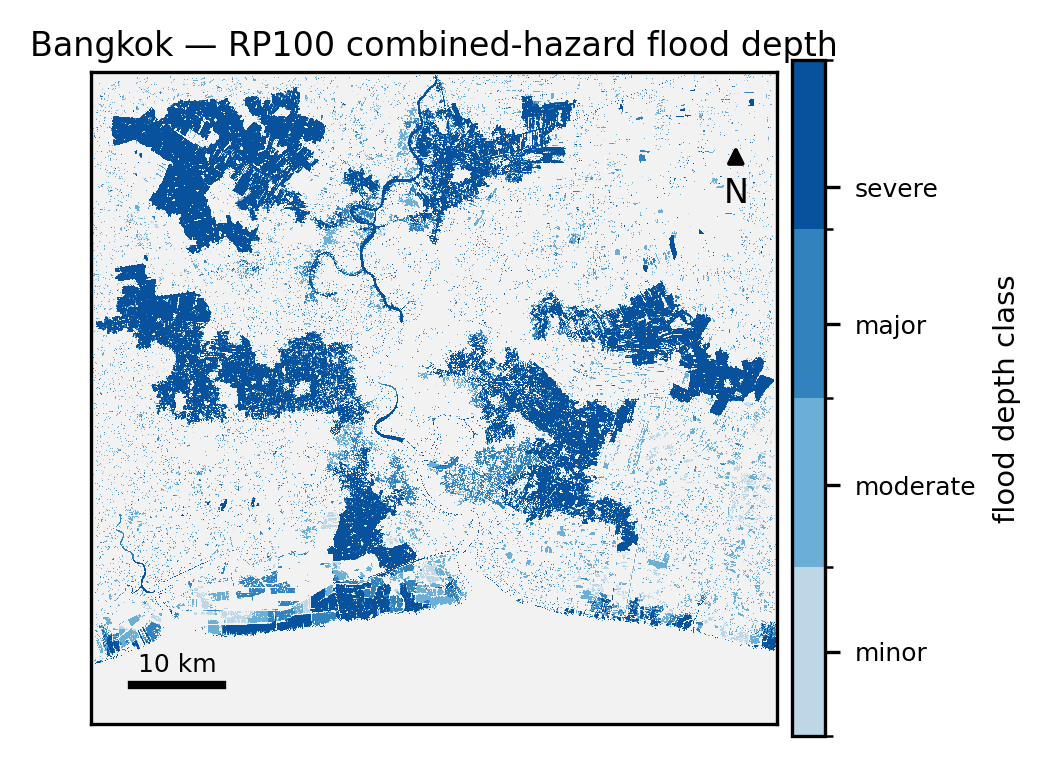
\includegraphics[width=\linewidth]{figures/ieee_fig2_bangkok_rp100.png}
\caption{Bangkok present-day-baseline RP100 combined-hazard flood-depth map (SSP5-8.5
forcing, 2020 horizon; $\sim$1{,}374\,km\textsuperscript{2} above 0.1\,m),
illustrating the screening flood envelope on the flat Chao Phraya delta. Depth
classes: minor (0.1--0.15\,m), moderate (0.15--0.5\,m), major (0.5--1\,m), severe
($>$1\,m).}
\label{fig:bangkok}
\end{figure}

\section{Validation and Trustworthiness}\label{sec:valid}
An open model is only useful if it can be trusted to flood where flooding actually
occurs. We test this directly with a \textbf{model-blind documented-hotspot
location-skill gate}. For each city we freeze, before consulting any model output, a
register of localities with \emph{documented} flooding (positives) and localities
documented to have stayed \emph{dry} (controls), each geocoded and DEM-verified. The
combined present-day wet mask (pluvial $\lor$ fluvial $\lor$ coastal,
$\geq$\,0.10\,m, within a 50\,m hit radius matching the geocoding precision) is scored
against the register at the event-matched RP100, reporting hit-rate (HR; sensitivity),
correct-reject-rate (CRR; specificity), and the Peirce--Hanssen--Kuipers true skill
statistic (TSS $=$ HR $+$ CRR $-$ 1) with a bootstrap 95\,\% confidence interval. The
register is a \emph{consistency check}: parameters are anchored upstream to documented
facts, and the gate is never used to retune them.

\begin{table}[t]
\centering
\caption{Documented-hotspot gate (present-day, RP100, $\geq$\,0.10\,m, 50\,m radius).}
\label{tab:hotspot}
\begin{tabular}{lccccl}
\hline
\textbf{City} & \textbf{pos/dry} & \textbf{HR} & \textbf{CRR} & \textbf{TSS [95\,\% CI]} & \textbf{verdict}\\
\hline
Kuala Lumpur & 17/7 & 0.76 & 0.86 & \textbf{0.62} [0.25, 0.88] & PASS\\
Singapore & 38/20 & 0.82 & 0.65 & \textbf{0.47} [0.21, 0.72] & fail-CRR\textsuperscript{\ddag}\\
Bangkok & 16/7 & 0.56 & 0.86 & \textbf{0.42} [0.04, 0.75] & fail-HR\\
Jakarta & 18/8 & 0.89 & 0.50 & \textbf{0.39} [0.03, 0.75] & fail-CRR\textsuperscript{\dag}\\
\hline
\end{tabular}\\[3pt]
\begin{minipage}{0.97\linewidth}\footnotesize
\textsuperscript{\ddag}Singapore is the city in which the gate was first developed; it
is scored here on the \emph{identical} basis as the other three, re-aligned from the
earlier pluvial-only\,/\,RP50\,/\,150\,m convention --- the model itself is unchanged.
Its 58-point register is the largest, its positives are PUB \emph{List of Flood-Prone
Areas} localities geocoded from road names (medium confidence, hence the conservative
50\,m radius), and its CRR shortfall is the combined RP100 wet mask catching low-lying
dry controls the deliberately conservative pluvial-only layer alone would spare.\\
\textsuperscript{\dag}Jakarta's TSS \emph{before} the model-blind reclassification of
two documented-flooded mislabels (Menteng, Gambir --- both inundated in 2007 and 2013)
was \textbf{0.16} (no skill); the reclassification is anchored to the flood record,
not the gate.
\end{minipage}
\end{table}

All four cities reach \textbf{statistically significant discriminative skill} ---
every TSS confidence interval excludes zero. The harness originated on Singapore and
transferred to Kuala Lumpur, Bangkok and Jakarta with no engine changes. Two findings
generalise. First, a \textbf{main-stem-HAND rule}: HAND must be referenced to the
trunk channel the modelled discharge represents (for Kuala Lumpur, the
$\geq$\,180\,km\textsuperscript{2} accumulation trunk), not a channel-initiation or
full-OSM network; doing so fixes a false-positive on a 60--77\,m hill by correct
physics and yields a credible floodplain, lifting Kuala Lumpur to CRR\,0.86\,/\,TSS\,0.62
(PASS). Second, a \textbf{dry-control discipline}: a genuine control that the model
floods stays in the register as a reported false positive, never dropped to pass; only
a control that is \emph{independently documented-flooded} is corrected --- Jakarta's
central-levee controls (Menteng, Gambir) sit on the Ciliwung corridor and are
documented inundated in 2007 and 2013, so reclassifying them on the flood-record
evidence (decided model-blind) lifts Jakarta from no-skill (TSS\,0.16) to significant
skill (TSS\,0.39). The remaining shortfalls are \emph{documented structural limits,
not tuning failures}: Bangkok's HR is bounded because the 2011 reference flood was
sourced from a catchment whose headwaters lie outside the model domain, and Jakarta's
residual specificity loss is fill-and-spill over-ponding on genuinely elevated ground.

A second, complementary result establishes that the open model's coastal layer is
corrected, not merely cheap. A bathtub solver --- the default in open screening tools
--- over-predicts documented present-day coastal inundation by \textbf{1.7--25$\times$
at RP100}, because 30\,m terrain cannot resolve the sub-pixel road raises, canals, and
bunds that protect small present-day events. Replacing it with the local-inertia
shallow-water solver, where the sea connects to the domain boundary, brings the
over-prediction to $\approx$1$\times$: Bangkok's RP100 coastal extent drops from
3{,}546\,km\textsuperscript{2} to \textbf{283\,km\textsuperscript{2} (a 12.5$\times$
reduction)}, within $\sim$30\,\% of the documented 2011 megaflood extent. The bias
correction is a solver-architecture fix, not a data limitation
(Fig.~\ref{fig:bias}). Two further checks are consistent and space-limited here: the
IDF-anchor re-derivation is exact (0 fails across all configurations), the documented
high-water-mark depth cross-check is in-band at three of five points, and satellite
extent-CSI is reported only as an observation-limited sanity check (urban SAR layover
and MODIS coarseness suppress the reference).

\begin{figure}[t]
\centering
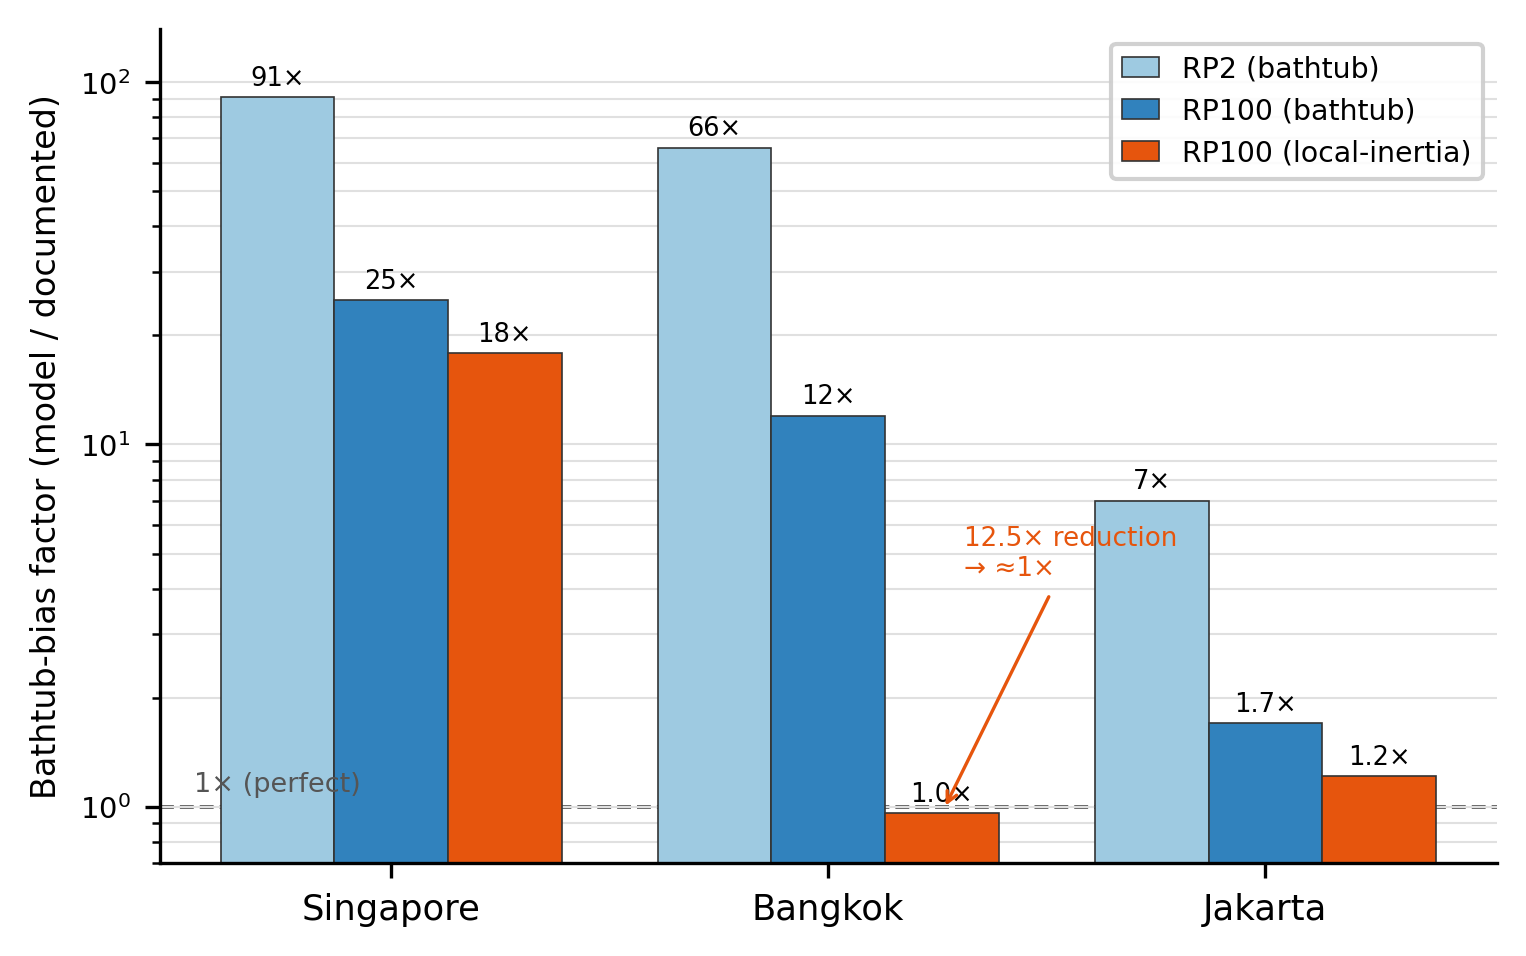
\includegraphics[width=\linewidth]{figures/ieee_fig3_bathtub_bias.png}
\caption{Bathtub-bias factor (model\,/\,documented) at RP2 and RP100 by city, with
the local-inertia overlay for the three solver-compatible cities (log scale). The
12.5$\times$ Bangkok RP100 reduction to $\approx$1$\times$ is the headline; Singapore's
residual ratio stays high because its documented present-day coastal extent is near
zero.}
\label{fig:bias}
\end{figure}

\section{Impact and Limitations}\label{sec:impact}
The intended use is humanitarian: open, validated, reproducible hazard maps as
decision-support for the municipal disaster-management and climate-adaptation agencies
that cannot license commercial models. Because every input is free and every parameter
is documented, an agency or a regional university can rebuild the atlas for its own
city, interrogate the assumptions, and extend it --- lowering the barrier to
first-order flood-risk information from a procurement question to a software install.

The model is honest as a \emph{screening upper bound} under three assumptions: no
active pumping, no sub-pixel defences resolved by the 30\,m DEM, and
per-pixel-maximum (marginal, not joint-exceedance) multi-hazard composition. The
scenario forcing is consistent across the full SSP\,$\times$\,horizon grid --- monotone
in scenario severity and within physical plausibility bounds, verified by an automated
consistency guard --- and the headline quantitative results use the validated
SSP5-8.5/2100 and present-day cells. Two further findings bound transferability and are
reported rather than tuned away: single-stage HAND does not transfer to flat deltas
fed by an out-of-domain mega-river (Bangkok, Jakarta), and the
pluvial solver is
currently heterogeneous across cities (a documented homogenisation step). The two
further ASEAN cities --- Manila (enclosed bay) and Ho Chi Minh City (enclosed delta)
--- are deferred because their enclosed-sea topology breaks the inertial solver's wall
condition; relaxing that condition is the principal prerequisite for extending the
bias-aware coastal treatment to them.

\section{Conclusion}
We have shown that an open-source, open-data, per-country-calibrated 30\,m
multi-hazard flood atlas for ASEAN cities is feasible, reproducible from free data,
and --- by a model-blind location-skill gate --- demonstrably skilful in the four
cities tested, with its coastal over-prediction structurally corrected. To our
knowledge it is the first such atlas released with full code, configuration, and
validation transparency for the region. By targeting exactly the cities that
commercial high-resolution models exclude, the release is offered as a public good for
humanitarian flood-risk reduction, and as an invitation to extend.

\section*{Reproducibility}
Code, per-city configuration, and the validation registers are released openly at
\url{https://github.com/phangdaniel-debug/ASEAN\_flood\_model}, enabling third-party
rebuild of every result from free data.

% References are ordered by first citation in the text (IEEE convention).
\begin{thebibliography}{99}
\bibitem{ref_adb} Asian Development Bank, ``Asia in the Global Transition to Net Zero:
Asian Development Outlook 2022 Thematic Report,'' 2022.
\bibitem{ref_lenderink} G. Lenderink, R. Barbero, J. M. Loriaux, and H. J. Fowler,
``Super-Clausius--Clapeyron Scaling of Extreme Hourly Convective Precipitation and
Its Relation to Large-Scale Atmospheric Conditions,'' \emph{J. Climate}, vol. 30,
pp. 6037--6052, 2017.
\bibitem{ref_chaussard} E. Chaussard, F. Amelung, H. Abidin, and S.-H. Hong,
``Sinking cities in Indonesia: ALOS PALSAR detects rapid subsidence,'' \emph{Remote
Sens. Environ.}, vol. 128, pp. 150--161, 2013.
\bibitem{ref_abidin} H. Z. Abidin \emph{et al.}, ``Land subsidence of Jakarta and its
relation with urban development,'' \emph{Nat. Hazards}, vol. 59, pp. 1753--1771, 2011.
\bibitem{ref_phienwej} N. Phien-wej, P. H. Giao, and P. Nutalaya, ``Land subsidence in
Bangkok, Thailand,'' \emph{Eng. Geol.}, vol. 82, pp. 187--201, 2006.
\bibitem{ref_hallegatte} S. Hallegatte, C. Green, R. J. Nicholls, and J.
Corfee-Morlot, ``Future flood losses in major coastal cities,'' \emph{Nat. Clim.
Change}, vol. 3, pp. 802--806, 2013.
\bibitem{ref_tellman} B. Tellman \emph{et al.}, ``Satellite imaging reveals increased
proportion of population exposed to floods,'' \emph{Nature}, vol. 596, pp. 80--86,
2021.
\bibitem{ref_fathom} O. E. J. Wing \emph{et al.}, ``A 30\,m global flood inundation
model for any climate scenario,'' \emph{Water Resour. Res.}, vol.~60,
e2023WR036460, 2024.
\bibitem{ref_hofste} R. W. Hofste, P. Reig, and L. Schleifer, ``Aqueduct 3.0: Updated
Decision-Relevant Global Water Risk Indicators,'' World Resources Institute, 2019.
\bibitem{ref_ward} P. J. Ward \emph{et al.}, ``Aqueduct Floods: global flood risk maps
and analysis,'' 2020.
\bibitem{ref_sutanudjaja} E. H. Sutanudjaja \emph{et al.}, ``PCR-GLOBWB 2: a 5\,arcmin
global hydrological and water resources model,'' \emph{Geosci. Model Dev.}, vol. 11,
pp. 2429--2453, 2018.
\bibitem{ref_era5land} J. Mu\~{n}oz-Sabater \emph{et al.}, ``ERA5-Land: a
state-of-the-art global reanalysis dataset for land applications,'' \emph{Earth Syst.
Sci. Data}, vol. 13, pp. 4349--4383, 2021.
\bibitem{ref_glofas} L. Alfieri \emph{et al.}, ``A global network for operational
flood risk reduction (GloFAS),'' \emph{Environ. Sci. Policy}, vol. 84, pp. 149--158,
2018.
\bibitem{ref_ar6} B. Fox-Kemper \emph{et al.}, ``Ocean, Cryosphere and Sea Level
Change,'' in \emph{Climate Change 2021: The Physical Science Basis (IPCC AR6 WGI)},
Cambridge Univ. Press, 2021.
\bibitem{ref_worldcover} D. Zanaga \emph{et al.}, ``ESA WorldCover 10\,m 2021 v200,''
Zenodo, 2022.
\bibitem{ref_ttide} R. Pawlowicz, B. Beardsley, and S. Lentz, ``Classical tidal
harmonic analysis including error estimates in MATLAB using T\_TIDE,'' \emph{Comput.
Geosci.}, vol. 28, pp. 929--937, 2002.
\bibitem{ref_muis2016} S. Muis, M. Verlaan, H. C. Winsemius, J. C. J. H. Aerts, and
P. J. Ward, ``A global reanalysis of storm surges and extreme sea levels,''
\emph{Nat. Commun.}, vol. 7, 11969, 2016.
\bibitem{ref_muis2020} S. Muis \emph{et al.}, ``A high-resolution global dataset of
extreme sea levels, tides, and storm surges, including future projections,''
\emph{Front. Mar. Sci.}, vol. 7, 263, 2020.
\bibitem{ref_bates} P. D. Bates, M. S. Horritt, and T. J. Fewtrell, ``A simple
inertial formulation of the shallow water equations for efficient two-dimensional
flood inundation modelling,'' \emph{J. Hydrol.}, vol. 387, no. 1--2, pp. 33--45, 2010.
\bibitem{ref_nobre} A. D. Nobre \emph{et al.}, ``Height Above the Nearest Drainage ---
a hydrologically relevant new terrain model,'' \emph{J. Hydrol.}, vol. 404, pp.
13--29, 2011.
\bibitem{ref_topo} C. D. Rennó, A. D. Nobre, L. A. Cuartas, J. V. Soares,
M. G. Hodnett, J. Tomasella, and M. A. Waterloo, ``HAND, a new terrain descriptor
using SRTM-DEM: Mapping terra-firme rainforest environments in Amazonia,''
\emph{Remote Sens. Environ.}, vol. 112, pp. 3469--3481, 2008.
\bibitem{ref_barnes} R. Barnes, K. L. Callaghan, and A. D. Wickert, ``Computing water
flow through complex landscapes --- Part 3: Fill--Spill--Merge,'' \emph{Earth Surf.
Dynam.}, vol. 9, pp. 105--121, 2021.
\bibitem{ref_planchon} O. Planchon and F. Darboux, ``A fast, simple and versatile
algorithm to fill the depressions of digital elevation models,'' \emph{Catena}, vol.
46, pp. 159--176, 2002.
\end{thebibliography}

\end{document}
